\documentclass[11pt,a4paper]{report}

\usepackage[polish]{babel}
\usepackage[utf8]{inputenc}
\usepackage[T1]{fontenc}
\usepackage{graphicx}
\usepackage{amsmath}
\usepackage[colorlinks=true, linkcolor=blue]{hyperref}
\usepackage{makeidx}
\usepackage{acronym}

\makeindex

\title{Polskie Potrawy Wigilijne}
\author{Marcin Piankowski, gr.3, 337882}
\date{\today}

\begin{document}
	
	\maketitle
	
	\tableofcontents
	\listoftables
	\listoffigures
	
	\sffamily
	\chapter*{Wstęp}
	Niniejszy dokument prezentuje najważniejsze potrawy, które powinny się znaleźć na stole wigilijnym w polsce 
	\rmfamily 
	
	\chapter{Tradycyjne Zupy Wigilijne}

\section{Barszcz czerwony z uszkami}
Wigilia w wielu regionach Polski, zwłaszcza na południu i wschodzie, tradycyjnie rozpoczyna się od barszczu czerwonego\index{Barszcz}. Zupa ta serwowana jest z drobnymi pierożkami faszerowanymi grzybami leśnymi, zwanymi uszkami\index{Uszka}. Opisuje to szczegółowo A. Nowak \cite{nowak2018}.

\section{Zupa grzybowa}
W centralnej i północnej części Polski na stołach częściej gości zupa grzybowa\index{Zupa grzybowa}, przygotowywana z suszonych borowików i podawana z domowym makaronem (tzw. łazankami).
	
	\chapter{Pierogi}
	
	\section{Pierogi z kapustą i grzybami}
	Pierogi to absolutna podstawa polskiej Wigilii.\index{Pierogi} Tradycyjnie przygotowuje się je z kiszoną kapustą i suszonymi grzybami leśnymi.
	
	\subsection{Tajemnica ciasta}
	Zgodnie z zaleceniami \ac{KGW}, idealne ciasto musi być elastyczne. \textit{Wyrabianie ciasta wymaga ciepłej wody i odrobiny cierpliwości} (przykład kursywy).
	
	\begin{figure}[ht]
		\centering
		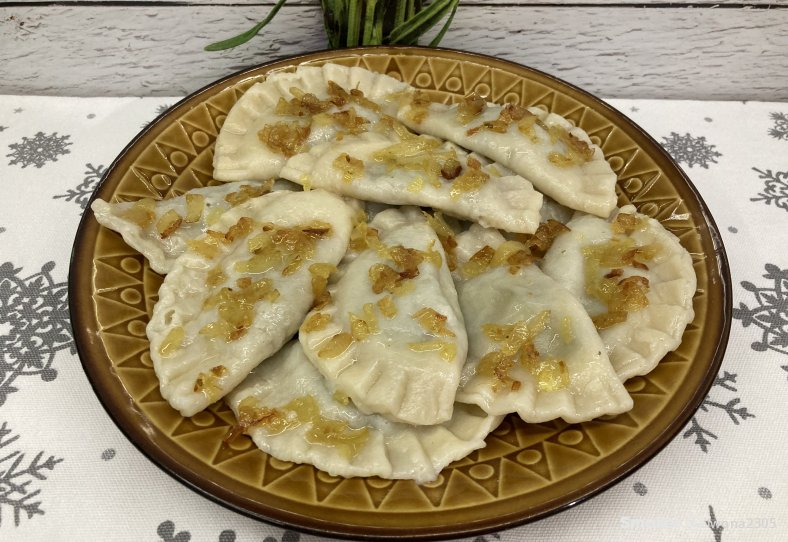
\includegraphics[width=0.5\textwidth]{pierogi.png}
		\caption{Tradycyjne pierogi wigilijne przed ugotowaniem}
		\label{fig:pierogi}
	\end{figure}
	
	Jak można zauważyć na rysunku \ref{fig:pierogi} (znajdującym się na stronie \pageref{fig:pierogi}), falbanka na krawędzi pełni funkcję dekoracyjną oraz praktyczną \cite{kowalski2020}.
	
	\newpage
	
	\section{Matematyka w kuchni}
	Aby precyzyjnie zaplanować przygotowania, musimy wyliczyć całkowitą masę ciasta i farszu $M$ (w gramach). W obliczeniach przyjmujemy liczbę gości $N$, średnią liczbę pierogów zjadanych przez jedną osobę $P$ oraz stały współczynnik $k$, który odpowiada średniej masie jednego pieroga (np. $k = 40$g).
	
	Wzór w tekście przyjmuje prostą postać iloczynu: $M = N \cdot P \cdot k$.
	
	Bardziej przejrzysty zapis matematyczny, pozwalający na szybkie oszacowanie potrzebnych składników bez zbędnych komplikacji, prezentuje równanie \ref{eq:prosta_masa}:
	\begin{equation}
		M = N \cdot P \cdot k
		\label{eq:prosta_masa}
	\end{equation}
	
	Gdzie:
	\begin{itemize}
		\item $M$ – całkowita masa potrawy [g],
		\item $N$ – liczba osób przy stole,
		\item $P$ – statystyczna liczba pierogów na osobę (zazwyczaj od 8 do 12),
		\item $k$ – średnia masa jednego pieroga w gramach.
	\end{itemize}
	
	Odwołanie do obliczeń: zgodnie z równaniem \ref{eq:prosta_masa} na stronie \pageref{eq:prosta_masa}, dla 10 gości zjadających po 10 pierogów o masie 40g, będziemy potrzebować 4 kg gotowego produktu.
	
	
	\chapter{Ryby na stole wigilijnym}
	\index{Ryby}
	Zgodnie z polską tradycją kulinarną, na stole nie może zabraknąć dań rybnych. 
	
	\begin{table}[ht]
		\centering
		\begin{tabular}{|l|c|c|}
			\hline
			\textbf{Gatunek ryby} & \textbf{Sposób przyrządzenia} & \textbf{Kaloryczność (kcal/100g)} \\
			\hline
			Karp & smażony, w galarecie & 130 \\
			Śledź & w oleju, w śmietanie & 160 \\
			Dorsz & po grecku & 82 \\
			\hline
		\end{tabular}
		\caption{Zestawienie popularnych ryb wigilijnych}
		\label{tab:ryby}
	\end{table}
	
	Szczegółowe wartości odżywcze zostały przedstawione w tabeli \ref{tab:ryby} na stronie \pageref{tab:ryby}.
	
	
	\appendix
	\chapter{Załączniki}
	\section{Przepis na przyprawę piernikową}
	\textbf{Składniki:} cynamon, goździki, gałka muszkatołowa, kardamon, imbir. Proporcje można dostosować do własnych preferencji (demonstracja tekstu pogrubionego).
	
	
	\chapter{Wykaz skrótów}
	\begin{acronym}[KGW]
		\acro{KGW}{Koło Gospodyń Wiejskich}
		\acro{PRL}{Polska Rzeczpospolita Ludowa}
	\end{acronym}
	
	
	\begin{thebibliography}{9}
		\bibitem{kowalski2020} Kowalski J., \emph{Polska Kuchnia Świąteczna. Tradycja i nowoczesność}, Wydawnictwo Kulinarne, Warszawa 2020.
		\bibitem{nowak2018} Nowak A., \emph{Zupy polskie}, Gdańsk 2018.
	\end{thebibliography}
	
	\printindex
	
\end{document}